\chapter{Evaluation}
As our study pursued an exploratory approach the evaluation was an experimental task. First we analysed both dependent variables seperatly
using our aggregated variables and functions from the previous chapter. We explored various transformations and looked for any statistical
significance based on the collected data. Regarding the answer time we also tried grouping the observations before building models to reduce the 
effect of outliers. Lastly we looked if there were any significant performance differences between
the groups of our four original study variables. The whole analysis was done using the R programming language and common packages. The code can be also
found on github: \url{https://github.com/SimonMeissner/geo-dashboard}.

\section{Answer time analysis}
Answer time will be analysed by formulating different linear regression and multiple linear regression models. As a measure for the quality of
the fitted models the adjusted $R^2$ value will be used. In summary, the adjusted R-squared is valuable not only for comparing models but also as a
standalone metric for assessing the fit of a linear regression model. It offers insights into the model's trade-off between explanatory power and
complexity, helps prevent overfitting, guides model selection, and promotes the development of models that are both accurate and interpretable.

As a starting point we wanted to look how our aggregated variables would correlate with the answer time if we use the theorized aggregated parameters
from the previous chapter. Because in the scope of our study the difficulty index was the only predictor regarding answer time we can directly look at the
linear pearson correlation coefficient of our three variables in \ref{difficultyIndexEquation} with the answer time.
The variable $\frac{1}{n_view}$ showed a positive correlation index of $0.08$, $\frac{1}{q_view}$ showed a positive correlation index of $0.33$
and the the distraction index showed a negative correlation index of $0.01$. Simple linear regressions with every variable in isolation showed following
adjusted R squared values: $\frac{1}{n_view} = -0.003$, $\frac{1}{q_view} = 0.096$ and $Index_{distraction} = -0.01$
A multiple linear regression with all three variables resulted in an adjusted $R^2$ value of $0.084$.


\subsection{Manipulating the view difficulty}
The first variable we manipulated was the calculation of the view distraction from equation \ref{viewDistractionEquation}. We used common
elementary functions to transform the impact of each view distraction. We always did the same tranformation to all four views. In our first model we followed a
linear development. Here we investigated how a power transformation, a logaritmic transformation and an exponential transformation would influence
the significance of the distraction index on the answer time. Table \ref{viewDistractionTransformations} shows all transformations that have
been explored, the pearson correlation index with the answer time variable and the adjusted $R^2$ from a linear regression with the transformed
view distraction values.

\begin{longtable}{| p{0.24\linewidth} | p{0.25\linewidth} | p{0.20\linewidth}|}
    \hline
    \textbf{Transformation} & \textbf{Correlation index} & \textbf{Adjusted $R^2$} \\
    \hline
    \endfirsthead
    \multicolumn{3}{l}{{\textit{Continued from previous page}}} \\
    \hline
    \textbf{Transformation} & \textbf{Correlation index} & \textbf{Adjusted $R^2$} \\
    \hline
    \endhead
    \hline \multicolumn{3}{r}{{\textit{Continued on next page}}} \\
    \endfoot
    \hline
    \caption{This table lists all transformations used for the view distraction in \ref{viewDistractionEquation}, the calculated correlation indices and the associated adjusted $R^2$ values \label{viewDistractionTransformations}}\\
    \endlastfoot
    $ \ln(x) $ & $0.00$ & -$0.011$ \\
    \hline
    $ \log_{2}(x) $ & $0.00$ & -$0.011$ \\
    \hline
    $ \log_{10}(x) $ & $0.00$ & -$0.011$ \\
    \hline
    $ \sqrt{x} $ & -$0.01$ & -$0.011$ \\
    \hline
    $ x^2 $ & $0.00$ & -$0.010$ \\
    \hline
    $ x^3 $ & $0.00$ & -$0.0$ \\
    \hline
    $ e^x $ & $0.34$ & $0.094$ \\
    \hline
    $ 2^x $ & $0.32$ & $0.094$ \\
    \hline
    $ 3^x $ & $0.34$ & $0.094$ \\
\end{longtable}

To further analyse we did multiple linear regressions with all exponential transformations. We included
$\frac{1}{n_{view}}$, $\frac{1}{q_{view}}$ and the distraction index with the transformed view distraction values for all four views. All three models
with $e^x$ transformation, $2^x$ transformation and $3^x$ transformation showed the same adjusted $R^2$ value of $0.14$.


\subsection{Manipulating the distraction index}
The second variable we manipulated was the distraction index from equation \ref{difficultyIndexEquation}. The view distraction of all four was again calculated
without any transformation. We tried the same variations of the three popular elementary function group transformations we used in the last transformation.
Table \ref{distractionIndexTransformations} shows the results.

\begin{longtable}{| p{0.24\linewidth} | p{0.25\linewidth} | p{0.20\linewidth}|}
    \hline
    \textbf{Transformation} & \textbf{Correlation index} & \textbf{Adjusted $R^2$} \\
    \hline
    \endfirsthead
    \multicolumn{3}{l}{{\textit{Continued from previous page}}} \\
    \hline
    \textbf{Transformation} & \textbf{Correlation index} & \textbf{Adjusted $R^2$} \\
    \hline
    \endhead
    \hline \multicolumn{3}{r}{{\textit{Continued on next page}}} \\
    \endfoot
    \hline
    \caption{This table lists all transformations used for the distraction index in \ref{distractionIndexEquation}, the calculated correlation indices and the associated adjusted $R^2$ values. \label{distractionIndexTransformations}}\\
    \endlastfoot
    $ \ln(x) $ & -$0.01$ & -$0.011$ \\
    \hline
    $ \log_{2}(x) $ & -$0.01$ & -$0.011$ \\
    \hline
    $ \log_{10}(x) $ & -$0.01$ & -$0.011$ \\
    \hline
    $ \sqrt{x} $ & -$0.01$ & -$0.011$ \\
    \hline
    $ x^2 $ & $0.01$ & -$0.010$ \\
    \hline
    $ x^3 $ & $0.04$ & -$0.0092$ \\
    \hline
    $ e^x $ & $0.30$ & $0.078$ \\
    \hline
    $ 2^x $ & $0.29$ & $0.076$ \\
    \hline
    $ 3^x $ & -$0.02$ & $0.078$ \\
\end{longtable}
The same multiple linear regression was done. We used all three variables with the new transformed distraction index. We again calculated three
models having the distraction index beeing transformed with $e^x$, $2^x$ and $3^x$. All three models displayed an adjusted $R^2$ value of $0.16$.

We also investigated the effect of transforming the distraction index as a whole while also transforming the view distraction.
Looking at table \ref{viewDistractionTransformations} we can see that an exponential transformation of the view distraction of all view
looks the most promising. We decided to observe only the exponential function with base: $e$.
The following table \ref{distractionIndexTransformationsWithTransformedViewDistraction} looks at the correlation indices and the adjusted $R^2$
values of the distraction index transformations with already transformed view distraction. Here we exclude the exponential functions and the power
functions having an rational exponent > $\frac{1}{2}$ functions because the numerical values got so huge that the native functions used for linear
regression returned unreasonable results and error messages. Irrespective of this, we no longer expected any meaningful results by further increasing
the values.

\begin{longtable}{| p{0.24\linewidth} | p{0.25\linewidth} | p{0.20\linewidth}|}
    \hline
    \textbf{Transformation} & \textbf{Correlation index} & \textbf{Adjusted $R^2$} \\
    \hline
    \endfirsthead
    \multicolumn{3}{l}{{\textit{Continued from previous page}}} \\
    \hline
    \textbf{Transformation} & \textbf{Correlation index} & \textbf{Adjusted $R^2$} \\
    \hline
    \endhead
    \hline \multicolumn{3}{r}{{\textit{Continued on next page}}} \\
    \endfoot
    \hline
    \caption{This table lists all transformations used for the distraction index in \ref{distractionIndexEquation}, the calculated correlation indices and the associated adjusted $R^2$ values. All linear regressions were done on the already ln-transformed view distraction values. \label{distractionIndexTransformationsWithTransformedViewDistraction}}\\
    \endlastfoot
    $ \ln(x) $ & -$0.03$ & -$0.0095$ \\
    \hline
    $ \log_{2}(x) $ & -$0.03$ & -$0.0095$ \\
    \hline
    $ \log_{10}(x) $ & -$0.03$ & -$0.0095$ \\
    \hline
    $ x^{\frac{1}{8}} $ & $0.27$ & -$0.065$ \\
    \hline
    $ x^{\frac{1}{4}} $ & $0.32$ & $0.092$ \\
    \hline
    $ \sqrt{x} $ or $ x^{\frac{1}{2}} $ & $0.32$ & $0.094$ \\
\end{longtable}

We also tried to validate the tranformations within multiple linear regressions with all variables. We chose to analyse the last two transformations
from table \ref{distractionIndexTransformationsWithTransformedViewDistraction} $x^{\frac{1}{4}}$ and $x^{\frac{1}{2}}$. Those tranformed distraction index values
also included the $e^x$ transformation of the view distraction values. Both multiple linear regression models contained adjusted $R^2$ values of $0.14$.

\subsection{Manipulating the difficulty index}
The last variable we tried to transform was the difficulty index from equation \ref{answerTimeEquation}. For this transformation we summed all three variables
$\frac{1}{n_{view}}$, $\frac{1}{q_{view}}$ and the distraction index and transformed the solution using our known exemplary elementary functions. Table
\ref{difficultyIndexTransformations} shows again the calculated correlation indices and adjusted $R^2$ values.
\begin{longtable}{| p{0.24\linewidth} | p{0.25\linewidth} | p{0.20\linewidth}|}
    \hline
    \textbf{Transformation} & \textbf{Correlation index} & \textbf{Adjusted $R^2$} \\
    \hline
    \endfirsthead
    \multicolumn{3}{l}{{\textit{Continued from previous page}}} \\
    \hline
    \textbf{Transformation} & \textbf{Correlation index} & \textbf{Adjusted $R^2$} \\
    \hline
    \endhead
    \hline \multicolumn{3}{r}{{\textit{Continued on next page}}} \\
    \endfoot
    \hline
    \caption{This table lists all transformations used for the difficulty index in \ref{answerTimeEquation}, the calculated correlation indices and the associated adjusted $R^2$ values \label{difficultyIndexTransformations}}\\
    \endlastfoot
    $ \ln(x) $ & -$0.01$ & -$0.011$ \\
    \hline
    $ \log_{2}(x) $ & -$0.01$ & -$0.011$ \\
    \hline
    $ \log_{10}(x) $ & -$0.01$ & -$0.011$ \\
    \hline
    $ \sqrt{x} $ & -$0.01$ & -$0.011$ \\
    \hline
    $ x^2 $ & $0.01$ & -$0.010$ \\
    \hline
    $ x^3 $ & $0.04$ & -$0.0091$ \\
    \hline
    $ e^x $ & $0.30$ & $0.078$ \\
    \hline
    $ 2^x $ & $0.29$ & $0.076$ \\
    \hline
    $ 3^x $ & -$0.02$ & $0.078$ \\
\end{longtable}
Because we modelled answer time to only have our one known predictor difficulty index there was no possibility for multiple linear
regression.
\subsection{Grouping the observations}
A common practice with measurements generated from different humans is to compute representative values of the dependent variable for groups of
observations because of the high variablity of performance across different individuums. Normaly the median is used as a representative value because
it is more robust compared to the mean (outliers do not have much effect) \citep*{Daszykowski.2007}. Because our study was designed in a way that
only two observations per variable combination were generated, calculating the mean and the median
on every unique variable combination will result in the same values. We had 96 total observations and 48 unique variable combinations. Two instances
for number of views (n = 2, n = 4), two instances of comparison targets (n = 2, n = 3), three interaction techniques (\textit{filtering},
\textit{highlighting\_1} and \textit{highlighting\_2}) and four question types (type1, type2, type3 and type4) resulting in 48 unique combinations
($2 * 2 * 3 * 4$).

We decided to compute two multiple linear regression models using all three variables and the grouped dataset using the mean (or median) of the answer
time. In the first model we used the formula for the distraction index how it was computed at the beginning of this chapter without any transformation.
The model showed an adjusted $R^2$ value of $0.084$. The second model implemented the most promising previous observations by using the transformation
that showed the highest adjusted $R^2$ value in the mulitple linear regression using all three variables. We decided to calculate a model that uses the
$3^x$ transformation for the distraction index. The model had an adjusted $R^2$ value of $0.18$. Running the smae multiple linear regression without the
$\frac{1}{n_{view}}$ variable resulted in an adjusted $R^2$ of $0.17$.

\subsection{Quality of view}
Because $\frac{1}{q_{view}}$ showed an linear correlation coefficient of $0.33$ with answer time we decided to look for statistical significance using
an anova test. To look for homoscedasticity as it is a precondition for anova we run the levene test. When performing an anova test using the untransformed
answer time values the levene test resulted in a p-value of $0.0080$. We rerun the anova test with log10-transformed answer time values and retrieved a p-value
of $0.17$. The conditions for homoscedasticity were met an the anova test showed a p-value of $0.00096$.

\section{Answer accuracy analysis}
Answer accuracy will be analysed by building multiple logistic regression models. We will look for any statistical significance between the independent
variables and the collected data about the accuracy.

\subsection{Manipulating the discriminability index}
Because we decided that the discriminability index is the only predictor for the answer accuracy we will focus on manipulating $a_1$ in formular
\ref{answerAccuracyEquation}. For that we concluded to research the same elementary function transformations which were used in the answer time
analysis. As a measurement to determine statistical significance we looked at the p-value of the associated discriminability index transformation
in the logistic regression. We also included the simple linear correlation index. Table \ref{discriminabilityIndexTransformation} shows
the results for every discriminability index transformation using the default untransformed distraction index.
The logistic regression with $a_1 = 1$ (no transformation) yielded a correlation index of -$0.02$ and a p-value of $0.82$.
\begin{longtable}{| p{0.24\linewidth} | p{0.25\linewidth} | p{0.20\linewidth}|}
    \hline
    \textbf{Transformation} & \textbf{Correlation index} & \textbf{p-value} \\
    \hline
    \endfirsthead
    \multicolumn{3}{l}{{\textit{Continued from previous page}}} \\
    \hline
    \textbf{Transformation} & \textbf{Correlation index} & \textbf{p-value} \\
    \hline
    \endhead
    \hline \multicolumn{3}{r}{{\textit{Continued on next page}}} \\
    \endfoot
    \hline
    \caption{This table lists all transformations used for the discriminability index in \ref{answerAccuracyEquation}, the calculated correlation indices and the associated p-values \label{discriminabilityIndexTransformation}}\\
    \endlastfoot
    $ \ln(x) $ & $0.01$ & $0.91$ \\
    \hline
    $ \log_{2}(x) $ & $0.01$ & $0.91$ \\
    \hline
    $ \log_{10}(x) $ & $0.01$ & $0.91$ \\
    \hline
    $ \sqrt{x} $ & -$0.01$ & $0.94$ \\
    \hline
    $ x^2 $ & -$0.05$ & $0.64$ \\
    \hline
    $ x^3 $ & -$0.06$ & $0.54$ \\
    \hline
    $ e^x $ & -$0.02$ & $0.81$ \\
    \hline
    $ 2^x $ & -$0.02$ & $0.81$ \\
    \hline
    $ 3^x $ & -$0.02$ & $0.81$ \\
\end{longtable}

\section{Analysis of study variables}
Lastly we wanted to find out about the statistical significance of the raw study variables that are not yet aggregated in continuous ratio-scaled
variables. Meaning number of views, number of comparison targets, question type and interaction technique. We performed
one-way anova tests for every variable regarding the independent ratio-scaled answer time variable. 
The anova test for the number of views resulted in an p-value of $0.41$.
The anova test for the number of comparison targets deliverd an p-value of $0.00012$, the test for the question type showed an p-value of
$1.68 \times 10^{-7}$ and the test for the interaction technique showed an p-value of $0.28$. Before running the anova tests, we tested for
homoscedasticity (equal variances across groups) using the levene test as this is a precondition for the anova test. The test revealed that
the the variances across groups of the number of comparison targets and the question type were not equal and the anova test had to be run on
log-transformed answer time values to reach homoscedasticity as a precondition. Graphically boxplots of all variables and all groups can be
seen in figure \ref{boxplotsStudyVariablesAnswerTimefigure}.

To measure the influence of the variables on the independent variable answer accuracy we could not use anova because it is not interval- or
ratio-scaled an is not continuous which is a precondition for anova. We decided to run the popular chi squared test to test for any statistical differences
across groups. The test between the number of views and answer accuracy and the test between the number of comparison targets and answer accuracy both
delivered an p-value of $0.39$. The test between the question type and the answer accuracy showed an p-value of $0.023$. Because
some of the expected cell frequencies in the contengency table of the question type and the accuracy were smaller than 5 we additionally run the fisher's
exact test with a resulting p-value of $0.039$. The chi squared test delivered an p-value of $0.34$. In the contengency table of the interaction
technique and the accuracy the expected cell frequencies also were sometimes smaller than 5 and we also run an fisher's exact test which resulted in
an p-value of $0.44$.

\begin{figure}[ht]
    \centering
    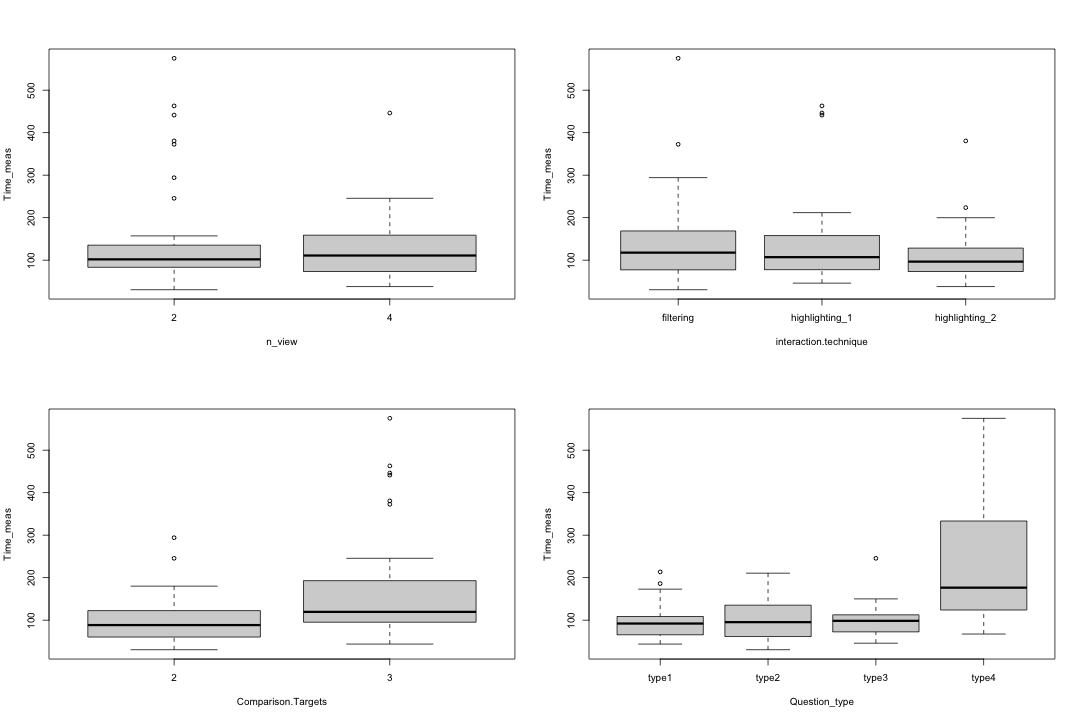
\includegraphics[width=15.5cm]{images/boxplots.png}
    \caption{Boxplots of all variables in the study and the answer time.} \label{boxplotsStudyVariablesAnswerTimefigure}
\end{figure}

\section{Subjective user feedback}
The study session was finalized with 3 questions regarding subjective feedback. The last question asked for the preferred dashboard variant of the
two used ones. Our sample size was 12 and the interaction techniques were balanced in a way that every interaction technique was used from four different
participants. Every technique was used two times on the first 4 questions and two times on the last four questions. Out of all participants 3 stated dashboard
variant 6 to be the favourable variant and also 3 selected variant 1 to be preferred. 2 participants each chose variant 3 and 4. And only one particpants
stated variant 2 to be preferred while also one chose variant 5. The mean expected selection count of each dashbaord variant was 2. We can conclude that
variants 2 and 5 were selected below average, the variants 3 and 4 were selected right on average and the variants 1 and 6 were selected above average to be
the preferred variant. Looking at the underlying interaction techniques of each dashboard we can derive that \textit{highlighting\_1} was preferred the least
because the related dashboard variants 2 and 5 were selected way below average. \textit{Filtering} and \textit{highlighting\_2} were both preferred the same
because variants 1 and 4 which realized \textit{filtering} and variants 3 and 6 which implemented \textit{highlighting\_2} both showed the same average pick rate.
Because the first two questions had an open nature to it is difficult to analyse the result. Various aspects were liked and disliked but many comments
regarded the clarity of the visualization and which was often times the main argument why they decided on a variant in question three. Also many participants
particularly disliked the additional rendering of the difference views and regarded it as distractive and as an contributor to an less clear understanding of
the dashboard.